

\tikzset{every picture/.style={line width=0.75pt}} %

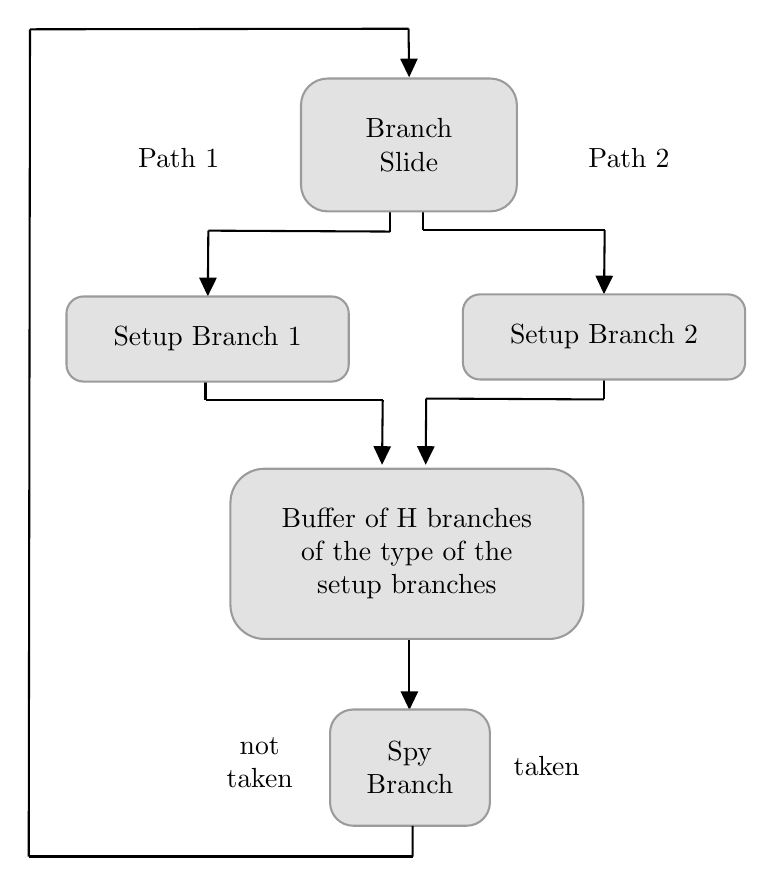
\begin{tikzpicture}[x=0.75pt,y=0.75pt,yscale=-1,xscale=1]

\draw    (343.22,537) -- (343.22,570.19) ;
\draw [shift={(343.22,573.19)}, rotate = 270] [fill={rgb, 255:red, 0; green, 0; blue, 0 }  ][line width=0.08]  [draw opacity=0] (8.93,-4.29) -- (0,0) -- (8.93,4.29) -- cycle    ;
\draw    (246.35,342.29) -- (246.12,370.88) ;
\draw [shift={(246.09,373.88)}, rotate = 270.46] [fill={rgb, 255:red, 0; green, 0; blue, 0 }  ][line width=0.08]  [draw opacity=0] (8.93,-4.29) -- (0,0) -- (8.93,4.29) -- cycle    ;
\draw    (246.35,342.29) -- (333.9,342.73) ;
\draw    (333.9,332.21) -- (333.9,342.73) ;

\draw    (349.94,342.09) -- (437.32,342.09) ;
\draw    (437.32,342.09) -- (437.02,369.91) ;
\draw [shift={(436.99,372.91)}, rotate = 270.61] [fill={rgb, 255:red, 0; green, 0; blue, 0 }  ][line width=0.08]  [draw opacity=0] (8.93,-4.29) -- (0,0) -- (8.93,4.29) -- cycle    ;
\draw    (349.94,331.82) -- (349.94,342.09) ;


\draw    (351.32,423.18) -- (351.09,452.07) ;
\draw [shift={(351.07,455.07)}, rotate = 270.45] [fill={rgb, 255:red, 0; green, 0; blue, 0 }  ][line width=0.08]  [draw opacity=0] (8.93,-4.29) -- (0,0) -- (8.93,4.29) -- cycle    ;
\draw    (351.32,423.18) -- (436.86,423.62) ;
\draw    (436.86,413) -- (436.86,423.62) ;

\draw    (245,423.96) -- (330.37,423.96) ;
\draw    (330.37,423.96) -- (330.08,452.07) ;
\draw [shift={(330.05,455.07)}, rotate = 270.59] [fill={rgb, 255:red, 0; green, 0; blue, 0 }  ][line width=0.08]  [draw opacity=0] (8.93,-4.29) -- (0,0) -- (8.93,4.29) -- cycle    ;
\draw    (245,413.6) -- (245,423.96) ;


\draw  [color={rgb, 255:red, 155; green, 155; blue, 155 }  ,draw opacity=1 ][fill={rgb, 255:red, 226; green, 226; blue, 226 }  ,fill opacity=1 ] (291,281.8) .. controls (291,274.73) and (296.73,269) .. (303.8,269) -- (382.2,269) .. controls (389.27,269) and (395,274.73) .. (395,281.8) -- (395,320.2) .. controls (395,327.27) and (389.27,333) .. (382.2,333) -- (303.8,333) .. controls (296.73,333) and (291,327.27) .. (291,320.2) -- cycle ;
\draw  [color={rgb, 255:red, 155; green, 155; blue, 155 }  ,draw opacity=1 ][fill={rgb, 255:red, 226; green, 226; blue, 226 }  ,fill opacity=1 ] (369,381.2) .. controls (369,376.67) and (372.67,373) .. (377.2,373) -- (496.8,373) .. controls (501.33,373) and (505,376.67) .. (505,381.2) -- (505,405.8) .. controls (505,410.33) and (501.33,414) .. (496.8,414) -- (377.2,414) .. controls (372.67,414) and (369,410.33) .. (369,405.8) -- cycle ;
\draw  [color={rgb, 255:red, 155; green, 155; blue, 155 }  ,draw opacity=1 ][fill={rgb, 255:red, 226; green, 226; blue, 226 }  ,fill opacity=1 ] (257,473.4) .. controls (257,464.34) and (264.34,457) .. (273.4,457) -- (410.6,457) .. controls (419.66,457) and (427,464.34) .. (427,473.4) -- (427,522.6) .. controls (427,531.66) and (419.66,539) .. (410.6,539) -- (273.4,539) .. controls (264.34,539) and (257,531.66) .. (257,522.6) -- cycle ;
\draw  [color={rgb, 255:red, 155; green, 155; blue, 155 }  ,draw opacity=1 ][fill={rgb, 255:red, 226; green, 226; blue, 226 }  ,fill opacity=1 ] (305,584.2) .. controls (305,578.01) and (310.01,573) .. (316.2,573) -- (370.8,573) .. controls (376.99,573) and (382,578.01) .. (382,584.2) -- (382,617.8) .. controls (382,623.99) and (376.99,629) .. (370.8,629) -- (316.2,629) .. controls (310.01,629) and (305,623.99) .. (305,617.8) -- cycle ;
\draw  [color={rgb, 255:red, 155; green, 155; blue, 155 }  ,draw opacity=1 ][fill={rgb, 255:red, 226; green, 226; blue, 226 }  ,fill opacity=1 ] (178,382.2) .. controls (178,377.67) and (181.67,374) .. (186.2,374) -- (305.8,374) .. controls (310.33,374) and (314,377.67) .. (314,382.2) -- (314,406.8) .. controls (314,411.33) and (310.33,415) .. (305.8,415) -- (186.2,415) .. controls (181.67,415) and (178,411.33) .. (178,406.8) -- cycle ;
\draw    (159.81,643.83) -- (344.81,643.83) ;
\draw    (342.8,245) -- (343.08,265.35) ;
\draw [shift={(343.12,268.35)}, rotate = 269.22] [fill={rgb, 255:red, 0; green, 0; blue, 0 }  ][line width=0.08]  [draw opacity=0] (8.93,-4.29) -- (0,0) -- (8.93,4.29) -- cycle    ;
\draw    (160.43,245.28) -- (159.81,643.83) ;

\draw    (342.8,245) -- (160.43,245.28) ;


\draw    (344.78,629.08) -- (344.81,643.83) ;



\draw (211,301) node [anchor=north west][inner sep=0.75pt]   [align=left] {\textbf{{\fontfamily{helvet}\selectfont Path 1}}};
\draw (428,301) node [anchor=north west][inner sep=0.75pt]   [align=left] {\textbf{{\fontfamily{helvet}\selectfont Path 2}}};
\draw (250,585) node [anchor=north west][inner sep=0.75pt]   [align=left] {\begin{minipage}[lt]{29.37pt}\setlength\topsep{0pt}
\begin{center}
\textbf{{\fontfamily{helvet}\selectfont not}}\\\textbf{{\fontfamily{helvet}\selectfont taken}}
\end{center}

\end{minipage}};
\draw (392,594) node [anchor=north west][inner sep=0.75pt]   [align=left] {\textbf{{\fontfamily{helvet}\selectfont taken}}};
\draw (342,498) node   [align=left] {\begin{minipage}[lt]{106.44pt}\setlength\topsep{0pt}
\begin{center}
\textbf{{\fontfamily{helvet}\selectfont Buffer of H branches }}\\\textbf{{\fontfamily{helvet}\selectfont of the type of the}}\\\textbf{{\fontfamily{helvet}\selectfont  setup branches}}
\end{center}

\end{minipage}};
\draw (343,301) node   [align=left] {\begin{minipage}[lt]{40.7pt}\setlength\topsep{0pt}
\begin{center}
\textbf{{\fontfamily{helvet}\selectfont Branch }}\\\textbf{{\fontfamily{helvet}\selectfont Slide}}
\end{center}

\end{minipage}};
\draw (437,393.5) node   [align=left] {\begin{minipage}[lt]{77.54pt}\setlength\topsep{0pt}
\begin{center}
\textbf{{\fontfamily{helvet}\selectfont Setup Branch 2}}
\end{center}

\end{minipage}};
\draw (246,394.5) node   [align=left] {\begin{minipage}[lt]{77.54pt}\setlength\topsep{0pt}
\begin{center}
\textbf{{\fontfamily{helvet}\selectfont Setup Branch 1}}
\end{center}

\end{minipage}};
\draw (343.5,601) node   [align=left] {\begin{minipage}[lt]{37.87pt}\setlength\topsep{0pt}
\begin{center}
\textbf{{\fontfamily{helvet}\selectfont Spy }}\\\textbf{{\fontfamily{helvet}\selectfont Branch}}
\end{center}

\end{minipage}};


\end{tikzpicture}
